\documentclass[9pt]{article}

\usepackage[margin=2cm]{geometry}
\usepackage{hyperref}
\usepackage{algorithm}
\usepackage{algpseudocode}
\usepackage{amsmath, amsthm, amssymb}
\usepackage{multicol, multirow}
\usepackage{tikz}
\usetikzlibrary{graphs}

\newtheorem{claim}{Claim}

\title{
    \textbf{ECO311: Game Theory} \\
    \textbf{\large{Bonus Question Solution}}
}
\author{
    \href{mailto:divyajeet21529@iiitd.ac.in}{\textbf{Divyajeet Singh (2021529)}}
}
\date{}

\begin{document}
\maketitle

\section*{Solution}
We are given a finite set of agents arranged in a network, where each agent can choose an action from the set $\{\textbf{0}, \textbf{1}\}$.
The agents follow a \textit{Principle of Majority} where each agent is better off choosing the same action chosen by at least half of its neighbors.
We exclude the cases where an agent has an even number of neighbors and exactly half of them choose either action.

\subsection*{Part 1.}
We now formalize the given problem as a strategic game.
Let $N = \{\textbf{1}, 2, \ldots, n\}$ be the set of agents, arranged in a known, undirected graph structure $G = (N, E)$ where $E \subset N \times N$ is the set of edges representing the neighbors of each agent.
For simplicity, we assume that the edge-set is non-empty, and there are no duplicate edges or self loops in the network.
Let $A_{i} = \{\textbf{0}, \textbf{1}\}$ be the set of actions available to agent $i \in N$.
Finally, we define the utility function\footnote{\textbf{Abuse of Notation:} The payoff of every agent is ultimately also dependent on the underlying network structure.
We denote this by $U_{i}(a_{i}, a_{-i} \mid G)$, as opposed to notating $G$ as an input to the utility function.}
$U_{i}: \times_{j \in N} A_{j} \rightarrow \mathbb{R}$ for each agent $i \in N$ as
\begin{equation}
    \label{utility}
    U_{i}(a_{i}, a_{-i} \mid G) = \begin{cases}
        \textbf{1} & \text{if } a_{i} = \Call{Mode}{N_{A}(i) := \{ a_{j} \in a_{-i} \mid (i, j) \in E \}} \\
        \textbf{0} & \text{otherwise}
    \end{cases}
\end{equation}
where $a_{-i}$ denotes the action profile excluding $i$ and $\Call{Mode}{S}$ denotes the element with the highest frequency in the set $S$.
Note that if $i$ does not have any incident edges, then $N_{A}(i)$ is empty.
Consequently, the mode is undefined, the agent by default gets a payoff of 0 for either action.
Then, $\Gamma = (N, \{A_{i}\}_{i \in N}, \{U_{i}\}_{i \in N})$ is the required strategic game, where the agents in $N$ are arranged as a graph $G = (N, E)$.

\subsection*{Part 2.}
Consider the action profile $\textbf{a}_{\textbf{0}} = (\textbf{0}, \textbf{0}, \dots, \textbf{0}) \in \times_{i \in N} A_{i}$, i.e. the action profile where all agents choose the action $\textbf{0}$.
\begin{claim}
    The action profile $\textbf{a}_{\textbf{0}}$ where $a_{i} = \textbf{0}$ for all $i \in N$ is a pure-strategy Nash equilibrium in $\Gamma$.
\end{claim}
\begin{proof}
    For the sake of contradiction, let us assume that the action profile $\textbf{a}_{\textbf{0}}$ is not a pure-strategy Nash equilibrium.
    Then, there exists some defaulter agent $j \in N$, who can benefit by unilateral deviation (i.e. has an incentive to switch to some other action; in this case, $\bar{a}_{j} = \textbf{1}$).
    Agent $j$ must have a non-empty set of neighbors, as otherwise, either action leads to a payoff of 0.
    Formally, the benefit of $j$ by unilateral deviation can be expressed as
    \begin{equation}
        \label{contradiction}
        U_{j}(\textbf{0}_{1}, \textbf{0}_{2}, \dots, \textbf{0}_{j-1}, \textbf{1}, \textbf{0}_{j+1}, \dots, \textbf{0}_{n} \mid G)
        \geq
        U_{j}(\textbf{0}_{1}, \textbf{0}_{2}, \dots, \textbf{0}_{j-1}, \textbf{0}, \textbf{0}_{j+1}, \dots, \textbf{0}_{n} \mid G)
    \end{equation}
    where the subscripts denote the indices.
    But, since all $a_{i} = \textbf{0}$ where $i \neq j$, then all (and thus, at least half of) the neighbors of $j$ have chosen $\textbf{0}$.
    This means that by the problem definition, it is more beneficial to choose $\textbf{0}$ than $\textbf{1}$, which is in-fact reflected in the utility function as
    \begin{align}
        \label{utility-0}
        U_{j}(\textbf{0}_{1}, \textbf{0}_{2}, \dots, \textbf{0}_{j-1}, \textbf{0}, \textbf{0}_{j+1}, \dots, \textbf{0}_{n} \mid G) &= 1 \\
        \label{utility-1}
        U_{j}(\textbf{0}_{1}, \textbf{0}_{2}, \dots, \textbf{0}_{j-1}, \textbf{1}, \textbf{0}_{j+1}, \dots, \textbf{0}_{n} \mid G) &= 0
    \end{align}
    where \eqref{utility-0} holds as $a_{j} = \textbf{0}$ is the mode action of the neighbors of $j$ in $a_{-j}$.
    Substituting \eqref{utility-0} and \eqref{utility-1} in \eqref{contradiction}, we get
    \begin{equation}
        0 \geq 1
    \end{equation}
    which is a clear contradiction.
\end{proof}
Alternatively and more intuitively, the action profile $\textbf{a}_{\textbf{0}}$ is a pure-strategy Nash equilibrium as every agent is selecting the same action, $\textbf{0}$.
This means that each agent $i$ having a non-empty set of neighbors chooses the mode action of its neighbors.
This results in a payoff of 1 for each of them.
For each agent $j$ with no neighbors, the choice of their action is arbitrary (since it inevitably results in a 0 payoff for them), and so, choosing $\textbf{0}$ is at least as good as choosing $\textbf{1}$.
Thus, the action profile $\textbf{a}_{\textbf{0}}$ is a pure-strategy Nash equilibrium. \\
Similarly, the action profile $\textbf{a}_{\textbf{1}} = (\textbf{1}, \textbf{1}, \dots, \textbf{1}) \in \times_{i \in N} A_{i}$ is also a pure-strategy Nash equilibrium in $\Gamma$.

\subsection*{Part 3.}
We want to construct a connected graph/network of $6 \leq n \leq 12$ agents such that there exists a pure-strategy Nash equilibrium where some agents choose $\textbf{0}$, while others choose $\textbf{1}$. \\
We require a graph where the each agent choosing $\textbf{0}$ is adjacent to \textit{many} agents choosing $\textbf{0}$, and vis-\`a-vis for $\textbf{1}$.
A natural choice can thus be two separate cliques only having a single edge between them.
In such a network, agents in one clique can choose $\textbf{0}$, while agents in the other clique can choose $\textbf{1}$.
Intuitively, this results in a Nash equilibrium, because an agent $c$ in clique $C$ has a majority of its neighbors in $C$.
Given that the other agents in $C$ choose a specific action $\textbf{x} \in A_{c}$, it is utilitarian for $c$ to also choose $\textbf{x}$.
\begin{figure}[htbp]
    \centering
    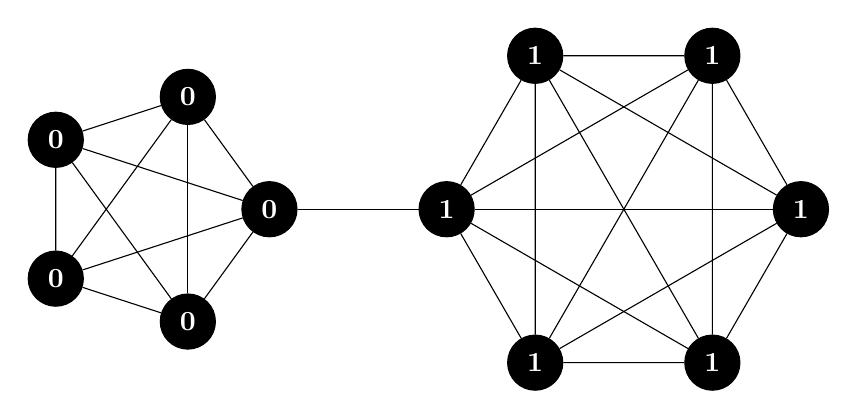
\begin{tikzpicture}[scale=1.5, every node/.style={circle, draw, fill=black, text=white, font=\bfseries, minimum size=7mm, inner sep=0pt}]
        \foreach \i in {1,...,5} {
            \node (K5-\i) at (\i*360/5:1) {$\textbf{0}$};
        }
        \foreach \i in {1,...,6} {
            \node (K6-\i) at (\i*360/6:1.5) [shift={(6,0)}] {$\textbf{1}$};
        }
        \foreach \i in {1,...,5} {
            \foreach \j in {1,...,5} {
                \ifnum\i<\j
                    \draw (K5-\i) -- (K5-\j);
                \fi
            }
        }
        \foreach \i in {1,...,6} {
            \foreach \j in {1,...,6} {
                \ifnum\i<\j
                    \draw (K6-\i) -- (K6-\j);
                \fi
            }
        }
        \draw (K5-5) -- (K6-3);
    \end{tikzpicture}
    \caption{A network of agents consisting of a $K_{5}$ and a $K_{6}$ connected via one edge.
    The action chosen by each agent is written on their corresponding node.}
    \label{fig:network}
\end{figure}
\vspace*{0pt} \\
Let $K_{i}$ denote the complete graph on $i$ vertices.
Figure \ref{fig:network} shows a network where a $K_{5}$ and a $K_{6}$ are connected by a single edge.
This arrangement results in $n = 11$ nodes.
It is easy to see that the graph is connected, i.e. there is a path between every pair of nodes.
\begin{claim}
    The action profile where the agents in $K_{5}$ choose $\textbf{0}$, while the agents in $K_{6}$ choose $\textbf{1}$, is a pure-strategy Nash equilibrium in $\Gamma$.
\end{claim}
\begin{proof}
    For the sake of contradiction, let us assume that the action profile in consideration is not a pure-strategy Nash equilibrium.
    Then, there exists some defaulter agent $j \in N$ with a non-empty set of neighbors, who can benefit by unilateral deviation.
    By construction, either $j \in K_{5}$ or $j \in K_{6}$.
    \vspace*{5pt} \\
    \textbf{Case 1.} $j \in K_{5}$, i.e. $a_{j} = \textbf{0}$.
    \begin{quote}
        \textbf{Case 1.1.} $j$ is connected to a node in $K_{6}$.
        Then, $j$ has 4 neighbors in $K_{5}$, all of whom have chosen $\textbf{0}$, and 1 neighbor in $K_{6}$.
        Since 4 out of 5 neighbors of $j$ have chosen $\textbf{0}$, $j$ does not benefit by deviation from $a_{j}$.
        \vspace*{3pt} \\
        \textbf{Case 1.2.} $j$ is not connected to a node in $K_{6}$.
        Then, all 4 neighbors of $j$ are in $K_{5}$ and have chosen $\textbf{0}$.
        So, $j$ does not benefit by deviation from $a_{j}$.
    \end{quote}
    \textbf{Case 2.} $j \in K_{6}$, i.e. $a_{j} = \textbf{1}$.
    \begin{quote}
        \textbf{Case 1.1.} $j$ is connected to a node in $K_{5}$.
        Then, $j$ has 5 neighbors in $K_{6}$, all of whom have chosen $\textbf{1}$, and 1 neighbor in $K_{5}$.
        Since 5 out of 6 neighbors of $j$ have chosen $\textbf{1}$, $j$ does not benefit by deviation from $a_{j}$.
        \vspace*{3pt} \\
        \textbf{Case 1.2.} $j$ is not connected to a node in $K_{5}$.
        Then, all 5 neighbors of $j$ are in $K_{6}$ and have chosen $\textbf{1}$.
        So, $j$ does not benefit by deviation from $a_{j}$.
    \end{quote}
    In all cases, $j$ does not benefit by deviation from their original action $a_{j}$, which is a contradiction to the assumption of $j$ being a defaulter.
\end{proof}


\end{document}